\documentclass[12pt]{article}
\usepackage{amsmath}
\usepackage{graphicx}
\usepackage{hyperref}
\usepackage{listings}
\usepackage{color}
\usepackage{pythonhighlight}

\title{Operating System Course Report - First Half of the Semester}
\author{B class}
\date{\today}

\begin{document}

\maketitle
\newpage

\tableofcontents
\newpage

\section{Introduction}
This report summarizes the topics covered during the first half of the Operating System course. It includes theoretical concepts, practical implementations, and assignments. The course focuses on the fundamentals of operating systems, including system architecture, process management, CPU scheduling, and deadlock handling.

\section{Course Overview}
\subsection{Objectives}
The main objectives of this course are:
\begin{itemize}
    \item To understand the basic components and architecture of a computer system.
    \item To learn process management, scheduling, and inter-process communication.
    \item To explore file systems, input/output management, and virtualization.
    \item To study the prevention and handling of deadlocks in operating systems.
\end{itemize}

\subsection{Course Structure}
The course is divided into two halves. This report focuses on the first half, which covers:
\begin{itemize}
    \item Basic Concepts and Components of Computer Systems
    \item System Performance and Metrics
    \item System Architecture of Computer Systems
    \item Process Description and Control
    \item Scheduling Algorithms
    \item Process Creation and Termination
    \item Introduction to Threads
    \item File Systems
    \item Input and Output Management
    \item Deadlock Introduction and Prevention
    \item User Interface Management
    \item Virtualization in Operating Systems
\end{itemize}

\section{Topics Covered}

\subsection{Basic Concepts and Components of Computer Systems}
This section explains the fundamental components that make up a computer system, including the CPU, memory, storage, and input/output devices.

\subsection{System Performance and Metrics}
This section introduces various system performance metrics used to measure the efficiency of a computer system, including throughput, response time, and utilization.

\subsection{System Architecture of Computer Systems}
Describes the architecture of modern computer systems, focusing on the interaction between hardware and the operating system.

\subsection{Process Description and Control}
\subsubsection{Definition of Process}
\subsubsection{Process states and state transitions}
\subsubsection{Process Control Block (PCB)}
\subsubsection{Context Switching}


\subsubsection{Process Management By Operating Systems}

\begin{figure}[h]
    \centering
    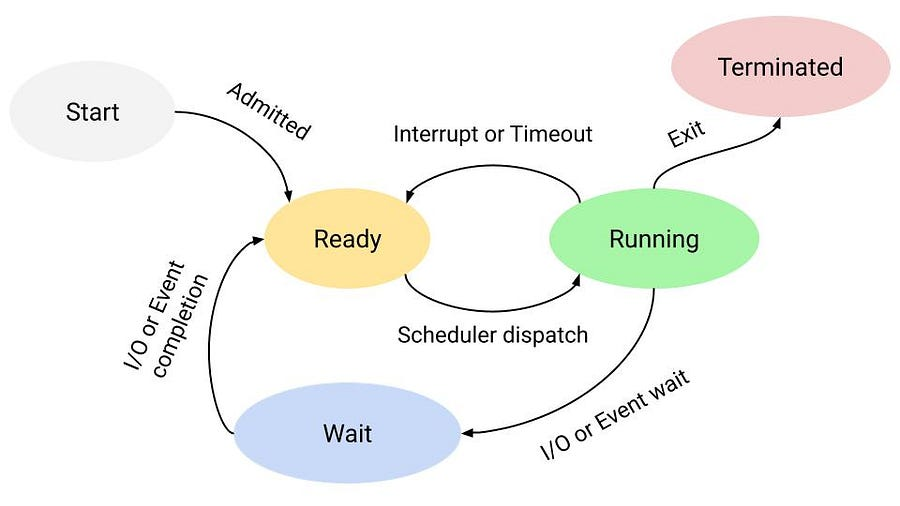
\includegraphics[width=0.5\textwidth]{assets/menejemen.jpg}  % Sesuaikan nama file dan ukurannya
    \caption{Ini adalah gambar contoh dari multithreading.}
    \label{fig:contoh_gambar}
\end{figure}
Manajemen proses oleh sistem operasi adalah salah satu tugas utama dari sistem operasi yang melibatkan pengelolaan dan pengendalian berbagai proses yang berjalan di komputer. Sistem operasi bertanggung jawab untuk memastikan bahwa proses-proses ini dieksekusi secara efisien dan tidak saling mengganggu. Berikut adalah aspek utama dari manajemen proses oleh sistem operasi:

\begin{itemize}
    \item \textbf{Pembuatan dan Penghancuran Proses}: 
   Sistem operasi membuat proses baru ketika suatu program dieksekusi atau ketika suatu proses meminta sistem untuk membuat subproses (misalnya dengan menggunakan perintah \textit{fork()} pada sistem UNIX). Saat proses dibuat, \textit{Process Control Block (PCB)} dialokasikan, dan informasi proses disimpan, termasuk ID proses, status proses, dan informasi lainnya. Sistem operasi juga bertanggung jawab untuk menghentikan dan menghapus proses yang telah selesai. Setelah proses selesai, sumber daya yang digunakan oleh proses dibebaskan agar bisa digunakan oleh proses lain.
    
    \item \textbf{Penjadwalan Proses (Process Scheduling)}: 
    Sistem operasi harus menentukan proses mana yang akan dijalankan terlebih dahulu, terutama dalam lingkungan multitasking di mana banyak proses berjalan secara bersamaan. Penjadwal Proses\textit{ (Scheduler) }menentukan urutan eksekusi proses berdasarkan prioritas dan status proses. Beberapa jenis penjadwalan proses yang umum meliputi:
    \begin{itemize}
        \item \textit{First Come First Serve }(FCFS): Proses yang datang terlebih dahulu akan dijalankan terlebih dahulu.
        \item \textit{Round Robin}: Setiap proses diberikan waktu eksekusi yang terbatas, kemudian berpindah ke proses lain.
        \item \textit{Shortest Job Next} (SJN): Proses dengan waktu eksekusi tersingkat dijalankan lebih dulu.
        \item \textit{Priority Scheduling}: Proses dengan prioritas lebih tinggi mendapatkan akses CPU lebih cepat.
    \end{itemize}
    
    \item \textbf{Context Switching}: 
    \textit{Context switching} adalah proses di mana CPU berpindah dari satu proses ke proses lain. Sistem operasi harus menyimpan konteks proses yang sedang berjalan (informasi register, \textit{program counter}, dll.) dan memuat konteks proses baru. Ini memungkinkan multitasking, di mana beberapa proses berjalan secara bersamaan (secara sekuensial tetapi sangat cepat sehingga tampak bersamaan).
    
    \item \textbf{Komunikasi Antar-Proses (\textit{Inter-Process Communication} - IPC)}: 
    Sistem operasi menyediakan mekanisme bagi proses untuk berkomunikasi satu sama lain, terutama jika mereka perlu berbagi data atau bekerja sama. Beberapa metode umum IPC termasuk:
    \begin{itemize}
        \item \textit{Shared Memory}: Dua atau lebih proses berbagi bagian dari memori.
        \item \textit{Message Passing}: Proses saling mengirim pesan untuk bertukar informasi.
    \end{itemize}
    
    \item \textbf{Sinkronisasi Proses}: 
    Sinkronisasi diperlukan untuk menghindari \textit{race conditions}, di mana dua proses mencoba mengakses atau memodifikasi sumber daya yang sama secara bersamaan. Mekanisme sinkronisasi yang disediakan oleh sistem operasi termasuk\textit{ semaphores, mutexes,} dan \textit{monitors.}
    
    \item \textbf{Manajemen Deadlock}: 
    Deadlock terjadi ketika dua atau lebih proses saling menunggu untuk sumber daya yang tidak bisa mereka peroleh, yang mengakibatkan proses tersebut tidak bisa melanjutkan eksekusi. Sistem operasi mengelola deadlock melalui berbagai strategi, seperti deteksi \textit{deadlock, }pencegahan \textit{deadlock}, atau penghindaran \textit{deadlock} (seperti algoritma Banker's).
    
    \item \textbf{Manajemen Sumber Daya Proses}: 
    Sistem operasi bertanggung jawab untuk mengalokasikan dan mengelola sumber daya yang dibutuhkan oleh proses, seperti CPU, memori, perangkat I/O, dan file. Ini termasuk memantau penggunaan sumber daya untuk mencegah konflik dan memastikan distribusi yang adil antara proses.
    
    \item \textbf{Keadaan Proses (Process States)}: 
    Setiap proses dalam sistem memiliki status tertentu (misalnya \textit{New, Ready, Running, Waiting, Terminated}) yang mencerminkan posisinya dalam siklus hidupnya. Sistem operasi bertanggung jawab untuk memindahkan proses antar status ini dan melakukan transisi secara efisien, seperti memindahkan proses dari \textit{ready} ke \textit{running} atau dari \textit{running} ke \textit{waiting.}
\end{itemize}

\subsection{Scheduling Algorithms}
This section covers:
\begin{itemize}
    \item First-Come, First-Served (FCFS)
    \item Shortest Job Next (SJN)
    \item Round Robin (RR)
\end{itemize}
It explains how these algorithms are used to allocate CPU time to processes.

\subsection{Process Creation and Termination}
Details how processes are created and terminated by the operating system, including:
\begin{itemize}
    \item Process spawning
    \item Process termination conditions
\end{itemize}

\subsection{Introduction to Threads}
This section introduces the concept of threads and their relation to processes, covering:
\begin{itemize}
    \item Single-threaded vs. multi-threaded processes
    \item Benefits of multithreading
\end{itemize}

\begin{figure}[h]
    \centering
    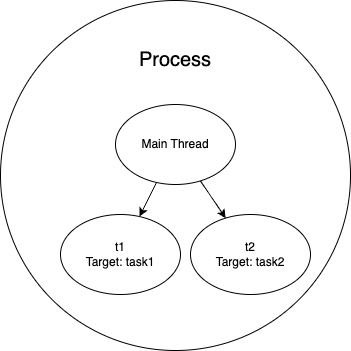
\includegraphics[width=0.5\textwidth]{assets/example.png}  % Sesuaikan nama file dan ukurannya
    \caption{Ini adalah gambar contoh dari multithreading.}
    \label{fig:contoh_gambar}
\end{figure}

Seperti yang terlihat pada Gambar \ref{fig:contoh_gambar}, inilah cara menambahkan gambar dengan keterangan.

\subsection{File Systems}
File systems provide a way for the operating system to store, retrieve, and manage data. This section explains:
\begin{itemize}
    \item File system structure
    \item File access methods
    \item Directory management
\end{itemize}

\subsection{Input and Output Management}
Input and output management is key for handling the interaction between the system and external devices. This section includes:
\begin{itemize}
    \item Device drivers
    \item I/O scheduling
\end{itemize}

\subsection{Deadlock Introduction and Prevention}
Explores the concept of deadlocks and methods for preventing them:
\begin{itemize}
    \item Deadlock conditions
    \item Deadlock prevention techniques
\end{itemize}

\subsection{User Interface Management}
This section discusses the role of the operating system in managing the user interface. Topics covered include:
\begin{itemize}
    \item Graphical User Interface (GUI)
    \item Command-Line Interface (CLI)
    \item Interaction between the user and the operating system
\end{itemize}

\subsection{Virtualization in Operating Systems}
Virtualization allows multiple operating systems to run concurrently on a single physical machine. This section explores:
\begin{itemize}
    \item Concept of virtualization
    \item Hypervisors and their types
    \item Benefits of virtualization in modern computing
\end{itemize}

\section{Assignments and Practical Work}
\subsection{Assignment 1: Process Scheduling}
Students were tasked with implementing various process scheduling algorithms (e.g., FCFS, SJN, and RR) and comparing their performance under different conditions.
\subsubsection{Group 1}
\begin{python}
    class Process:
    def __init__(self, pid, arrival_time, burst_time):
        self.pid = pid
        self.arrival_time = arrival_time
        self.burst_time = burst_time
        self.completion_time = 0
        self.turnaround_time = 0
        self.waiting_time = 0
\end{python}

\begin{table}[htbp] % Optional: For floating position
    \centering
    \begin{tabular}{|c|c|c|} % Defines number of columns and alignment (c = center, l = left, r = right). '|' creates vertical lines.
    \hline
    Header 1 & Header 2 & Header 3 \\ % Column headers
    \hline
    Row 1, Column 1 & Row 1, Column 2 & Row 1, Column 3 \\ % First row of data
    \hline
    Row 2, Column 1 & Row 2, Column 2 & Row 2, Column 3 \\ % Second row of data
    \hline
    \end{tabular}
    \caption{Your table caption} % Optional: For adding a caption
    \label{tab:your_label} % Optional: For cross-referencing the table
\end{table}

\subsection{Assignment 2: Deadlock Handling}
In this assignment, students were asked to simulate different deadlock scenarios and explore various prevention methods.

\subsection{Assignment 3: Multithreading and Amdahl's Law}
This assignment involved designing a multithreading scenario to solve a computationally intensive problem. Students then applied \textbf{Amdahl's Law} to calculate the theoretical speedup of the program as the number of threads increased.

\subsubsection{Group 4}
Apa itu \textbf{Hukum Amdahl} dan bagaimana hukum ini diterapkan dalam skenario multithreading untuk menghitung peningkatan kecepatan teoritis dari sebuah program?

\subsubsection{Jawaban}
Amdahl's Law adalah prinsip dalam komputasi paralel yang digunakan untuk memperkirakan peningkatan kinerja (speedup) suatu program ketika dijalankan secara paralel menggunakan beberapa thread atau prosesor. Menurut Amdahl's Law, peningkatan kinerja maksimal yang dapat dicapai oleh suatu program menggunakan pemrosesan paralel dibatasi oleh bagian dari program yang tidak dapat diparalelkan.

Amdahl's Law diwakili oleh rumus:

\[
S(N) = \frac{1}{(1 - P) + \frac{P}{N}}
\]

di mana:
\begin{itemize}
    \item $S(N)$ adalah speedup teoritis dengan $N$ thread.
    \item $P$ adalah persentase bagian dari program yang dapat diparalelkan.
    \item $N$ adalah jumlah thread atau prosesor yang digunakan.
\end{itemize}

Dalam skenario multithreading, Amdahl's Law membantu menghitung speedup teoritis dari program yang intensif secara komputasi seiring bertambahnya jumlah thread. Semakin besar bagian dari program yang dapat diparalelkan ($P$), semakin besar potensi peningkatan kinerja, tetapi peningkatan kinerja ini akan selalu dibatasi oleh bagian dari program yang tidak dapat diparalelkan.

\begin{itemize}
    \item {Python Code Implementation}
\end{itemize}

Kode Python berikut ini menunjukkan penerapan \textbf{Hukum Amdahl} untuk menghitung peningkatan kecepatan teoritis berdasarkan jumlah thread yang digunakan:

\begin{python}
def amdahls_law(P, N):
    """
    Menghitung speedup teoritis menggunakan Amdahl's Law.
    
    P : float : Persentase bagian yang bisa diparalelkan (0 <= P <= 1)
    N : int : Jumlah thread atau prosesor
    """
    if N == 0:
        return 1  # Tidak ada thread tambahan, jadi speedup tetap 1 (tidak ada paralelisme)
    
    return 1 / ((1 - P) + (P / N))

# Bagian yang bisa diparalelkan (misalnya 70\% dari program bisa diparalelkan)
P = 0.7

# Daftar jumlah thread yang akan diuji
threads = [1, 2, 4, 8, 16, 32]  

# Menghitung dan menampilkan speedup untuk setiap jumlah thread
for N in threads:
    speedup = amdahls_law(P, N)
    print(f"Jumlah thread: {N}, Speedup teoritis: {speedup:.2f}")
\end{python}

\begin{itemize}
    \item {Example Output}
\end{itemize}
Menggunakan implementasi \textit{Python} dari \textbf{Hukum Amdahl} dengan \( P = 0.7 \) (yaitu, 70\% dari program dapat diparalelkan) dan menguji peningkatan kecepatan dengan jumlah thread yang berbeda, kami mendapatkan hasil berikut:

\[
\begin{array}{|c|c|}
\hline
\text{Number of Threads} & \text{Theoretical Speedup} \\
\hline
1 & 1.00 \\
2 & 1.54 \\
4 & 2.11 \\
8 & 2.58 \\
16 & 2.91 \\
32 & 3.11 \\
\hline
\end{array}
\]

Seperti yang ditunjukkan oleh hasil, meningkatkan jumlah thread meningkatkan kecepatan, tetapi ada batasan pada peningkatan berdasarkan \textbf{Hukum Amdahl}. Bahkan dengan 32 thread, kecepatan maksimum yang dicapai adalah sekitar 3.11, karena 30\% dari program tidak dapat diparalelkan.



\subsection{Assignment 4: Simple Command-Line Interface (CLI) for User Interface Management}
Students were tasked with creating a simple **CLI** for user interface management. The CLI should support basic commands such as file manipulation (creating, listing, and deleting files), process management, and system status reporting.

\subsection{Assignment 5: File System Access}
In this assignment, students implemented file system access routines, including:
\begin{itemize}
    \item File creation and deletion
    \item Reading from and writing to files
    \item Navigating directories and managing file permissions
\end{itemize}

\section{Kesimpulan}
Laporan ini mengulas dasar-dasar sistem operasi, meliputi arsitektur sistem, manajemen proses, penjadwalan CPU, dan penanganan \textit{deadlock}. Materi yang dipelajari memberikan wawasan mendalam tentang cara kerja sistem operasi dan pentingnya komunikasi antar-proses serta sinkronisasi untuk menghindari kondisi balapan dan \textit{deadlock}. Konsep multithreading dan penerapan Hukum Amdahl juga menyoroti keuntungan pemrograman paralel dalam meningkatkan kinerja. Secara keseluruhan, pemahaman ini mempersiapkan mahasiswa menghadapi tantangan di dunia nyata serta membangun fondasi yang kuat untuk pengembangan perangkat lunak dan penelitian di masa depan.


%\section*{Daftar Pustaka}

\begin{thebibliography}{}

\bibitem{}
GeeksforGeeks. (n.d.). \textit{Process states in operating system}. Diakses pada 30 September 2024, dari \url{https://www.geeksforgeeks.org/process-states-in-operating-system/}

\bibitem{}
Tutorialspoint. (n.d.). \textit{Operating system - Process control block}. Diakses pada 30 September 2024, dari \url{https://www.tutorialspoint.com/operating_system/os_process_control_block.htm}

\bibitem{}
Wikipedia contributors. (n.d.). Context switch. Dalam \textit{Wikipedia, The Free Encyclopedia}. Diakses pada 30 September 2024, dari \url{https://en.wikipedia.org/wiki/Context_switch}

\end{thebibliography}

\end{document}